\subsection{Konzeptionelle und Organisatorische Aufgaben}
In diesem Abschnitt finden sich Aufgaben konzeptioneller sowie organisatorischer Natur, die sich mit dem Software-Entwicklungsprozess beschäftigt haben.

\subsubsection{Pflege eines schemenhaften Klassendiagramms}
Um die Struktur unseres Programmes grob zu visualisieren und so eine bessere Orientierung im Code zu ermöglichen sowie einen einheitlichen Wissensstand unter allen Beteiligten zu etablieren, erarbeitete und pflegte Felix Baumgarten ein Klassendiagramm.

Dieses half unter anderem, die Aufgabenverteilung mittels Git-Branches und die Kapselungsorganisation zu vereinfachen. Während der Arbeit am Projekt wurde das Diagramm an einem Whiteboard abgebildet und ergänzt, da Änderungen schnell umzusetzen waren und wir uns Einarbeitungszeit in komplexere digitale UML-Diagramme sparen wollten.
Eine Skizze des deutlich detaillierteren, da unter anderem mit Kardinalitäten ausgestatteten Klassendiagrams:
\begin{figure}[h]
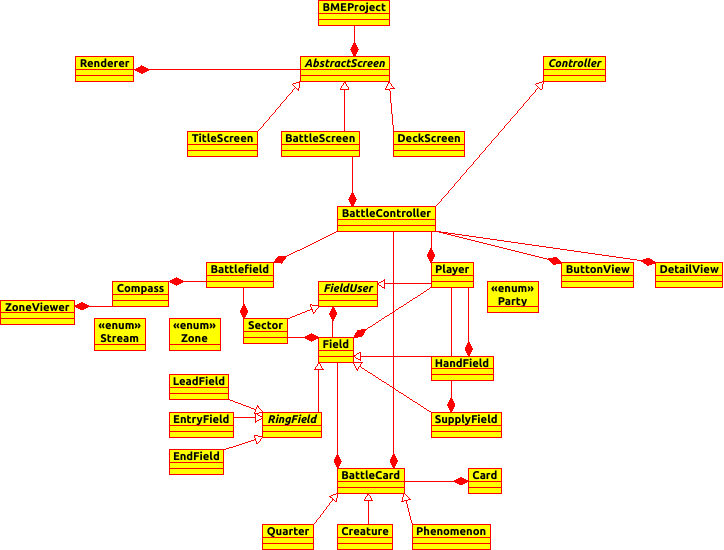
\includegraphics[width=1\textwidth]{../img/klassendiagramm.PNG}
\caption{Klassendiagramm Edwards Biotope}
\label{fig:Klassendiagramm_Edwards_Biotope}
\end{figure}